\documentclass[abstracton]{scrreprt}
\usepackage{style}
\begin{document}
\begin{titlepage}
\begin{center}

% Oberer Teil der Titelseite:
\textsc{\LARGE Technische Hochschule Köln}\\[1.5cm] % Name of your university/college
\textsc{\Large Mensch-Computer-Interaktion - Softwaretechnik 2}\\[0.5cm] % Major heading such as course name
\textsc{\large Praktikumsgruppe 13}\\[0.5cm] % Minor heading such as course title

% Title
\newcommand{\HRule}{\rule{\linewidth}{0.5mm}}
\HRule \\[0.4cm]
{ \huge \bfseries Portfolio: Campus Compass}\\[0.4cm]
\HRule \\[1.5cm]
\begin{minipage}{0.3\textwidth}
\begin{flushleft} \large
\emph{Autor:}\\
\textsc{Janis Saritzoglou}
\end{flushleft}
\end{minipage}
\hfill

\vfill
% Unterer Teil der Seite
{\large \today}
\end{center}
\end{titlepage}
\renewcommand\abstractname{Expos\'{e}}
\begin{abstract}
In der folgenden Arbeit wird konzipiert, wie ein plattformunabhängiges Indoor Navigations System für den Campus Gummersbach der FH-Köln für mobile Endgeräte und Tablets entworfen und implementiert werden kann.

\noindent
Der Fokus wird sich hierbei einerseits auf das Erstellen eines konsistenten und portierbaren Softwaremodelles und andererseits auf die bestmögliche Bedienbarkeit der Nutzer\-oberfläche richten.

\noindent
Weitere Herausforderungen im Bezug auf die Bedienbarkeit und die Wegfindung ergeben sich durch den Anspruch auch seh-- und gehbehinderte Nutzer zu unterstützen.
\end{abstract}
\tableofcontents
\listoffigures
\chapter{Nutzungskontext}
Bei der Analyse des Nutzungskontextes wird zunächst auf die beteiligten Personen und Gruppen eingegangen um anschließend zu untersuchen, mit welchen Erwartungen sie in welchen Szenarien an die Anwendung herantreten.

\subsubsection*{Problemraum}
Als \gls{ausgang}szustand, gibt es einen \gls{fhbesucher} der hat das Ziel einen \gls{ort} aufgrund einer seinerseits bestehenden \gls{intention}, zu erreichen. Um dieses Ziel zu erreichen sind Aufgaben/Aktivitäten, auch Operationen genannt, nötig. Im konkreten Fall der Indoor-\gls{navigation} sind diese Aufgaben/Aktivitäten Positionswechsel, welche der Anwender mit Hilfe der App, zu Fuß erledigen muss. Sind alle Teilschritte vom Anwender erledigt worden, erreicht der Anwender den Endzustand, den \gls{ort} an dem er seine \gls{intention} erfüllen kann.

\subsubsection*{Anwender (Akteure)}
\begin{itemize}
  \item Studenten
  \item Mitarbeiter der FH Koeln (extern/intern)
  \item Besucher/Fremde
\end{itemize}

\noindent
Die Anwender lassen sich allerdings auch auf andere Kategorien aufteilen, welche ihre für die Anwendung relevanten Eigenschaften besser abbilden.
\begin{itemize}
  \item Junge/Gesunde Menschen
  \item Alte Menschen
  \item Menschen mit und ohne Deutschkenntnisse
  \item Kranke/Verletzte Menschen
  \item Sehbehinderte Menschen
  \item Rollstuhlfahrer
\end{itemize}

\noindent
Ein wesentlicher Punkt ist das sich die verschiedenen Kategorien überlappen, es könnte beispielsweise ein Rollstuhlfahrer mit eingeschränkten Deutschkenntnissen den Wunsch haben, sich in der Fachhochschule navigieren zu lassen.

\subsubsection*{Stakeholder}
\begin{itemize}
  \item Dozenten/Auftraggeber
  \item Am Projekt beteiligte Studenten
\end{itemize}

\subsubsection*{Mentale Modelle}
Ein weiteres wichtiges Werkzeug in der Mensch-\-Computer-\-Interaktion ist der Einsatz von \emph{mentalen Modellen}, welche die Handlungen von Menschen aufgrund von Vorstellungen, Denkstrukturen und Erwartungen, welche sich im menschlichen Gedächtnisses befinden, beeinflussen und lenken.\medskip

\noindent Der User erwartet...
\begin{itemize}
  \item dass die \gls{navigation}sanwendung ihn \gls{schritt} für \gls{schritt} an sein Ziel führt und ihm visuell und akustisch mitteilt wie er ans Ziel gelangt bzw. wie er seinen nächsten \gls{schritt} macht. Ein Teilschritt kann auch als eine Aufgabe oder Aktivität zum erreichen des Ziels (An einen \gls{ort} gelangen, um eine \gls{intention} zu erfüllen) angesehen werden.
  \item \textbf{nicht}, dass er sein Ziel anhand eines abgebildeten \gls{weg}es auf einer 2D-Karte finden muss
  \item dass er auf Hindernisse auf seiner Zielroute hingewiesen wird und bei einer Blockade eine alternative Route geliefert bekommt
  \item dass er \gls{ort}e auch nach Bezeichnungen oder ihrem Zweck suchen kann (\gls{mensa}, WC, \dots)
\end{itemize}

\subsubsection*{Persona}
Personas stellen Prototypen für Gruppen von Nutzern mit konkret ausgeprägten Eigenschaften und einem konkreten Nutzungsverhalten dar. Sie werden später genutzt um User-Stories zu definieren.

\begin{itemize}
  \item \textbf{Max Meister (25)}, Informatikstudent im 4. Semester, keine physischen Einschränkungen
  \item \textbf{Hans Herd (64)}, Firmenvertreter, Besucher an der FH, Rollstuhlfahrer
  \item \textbf{Hubert Glücklich (20)}, Ingenieurwissenschaftenstudent, vor kurzem ein Bein gebrochen
  \item \textbf{Peter Redemann (44)}, Dozent an der FH, Blind
  \item \textbf{Ali Atas (26)}, Informatik-Austauschstudent, hat sehr eingeschränkte deutsche Sprachkenntnisse
  \item \textbf{Jürgen Watt (44)}, externer Elektriker, nutzt einen Werkzeugwagen 
\end{itemize}

\subsubsection*{User-Stories}
Basierend auf speziellen Eigenschaften der zuvor konkretisierten User Profiles (Persona), sind im folgenden User-Stories definiert.
\begin{itemize}
\item Als \gls{fhbesucher} möchte ich mein Profil festlegen, um trotz meinen ggf. körperlichen Einschränkungen ans einen Zielort gelangen zu können.
\item Als \gls{fhbesucher} möchte ich \gls{weg}optionen wählen können, um unabhängig von meinem festgelegten Profil alternative Routen wählen zu können. (Beispiel: User ist faul oder temporär physich eingeschränkt)
\item Als \gls{fhbesucher} möchte ich einen Zielort wählen können, um auch unabhängig von \gls{raum}nummern an einen \gls{ort} gelangen zu können.
\item Als \gls{fhbesucher} möchte ich auch dann ans Ziel gelangen, wenn mir die \gls{raum}nummer nicht bekannt ist, dazu möchte ich ein Anliegen auswählen.
\item Als \gls{fhbesucher} mit entsprechendem Profil möchte ich meine Anliegen statt von Hand auch per Spracheingabe eingeben können
\end{itemize}

\subsubsection*{Szenarien}
\begin{enumerate}
  \item Max Meister hat heute IM-Praktikum, das Praktikum findet in R1234 statt, er hat die \gls{raum}nummer im Stundenplan nachgeschaut und möchte sich nun bequem dorthin navigieren lassen. Max startet nun die \gls{navigation}sanwendung auf seinem Smartphone und tippt die \gls{raum}nummer ein. Nun startet er die \gls{navigation}.
  \item Peter Redemann muss gleich eine Vorlesung halten, das Semester hat gerade erst begonnen und seine Vorlesung findet nun in einem anderen, ihm nicht gewohnten \gls{raum} statt. Um den \gls{raum} zu finden möchte er die \gls{navigation}sanwendung auf seinem Smartphone nutzen. Er startet also die \gls{navigation}s-App und nennt die \gls{raum}nummer, welche via Spracheingabe erfasst wird. Mit den Worten “\gls{navigation} jetzt starten”, wird er nun per Sprachausgabe an sein Ziel geführt.
  \item Jürgen Watt hat den Auftrag einige Lampen im dritten Stock zu tauschen, er war noch nie am Campus Gummersbach und weiß deshalb nicht wo es lang geht. Er fährt auf den Parkplatz des Campus, geht durch den Haupteingang hinein und stellt fest, dass er mit seinem schweren Werkzeugwagen nicht die \gls{treppe}n hinauf kommt. Um eine alternative Route zu finden, startet er die \gls{navigation}sapp und trägt den ersten der ihm genannten Räume ein. Um nicht die \gls{treppe}n nutzen zu müssen, verbietet er in den \gls{weg}optionen die \gls{treppe}n.
\end{enumerate}

\subsubsection*{Use Case Diagramm (Verhalten)}
... bietet eine standardisierte Möglichkeit um die zuvor genannten Nutzer und ihre Use Cases sowie die Beziehungen zwischen Use Cases untereinander darzustellen.

\begin{figure}[hbt]
  \centering
  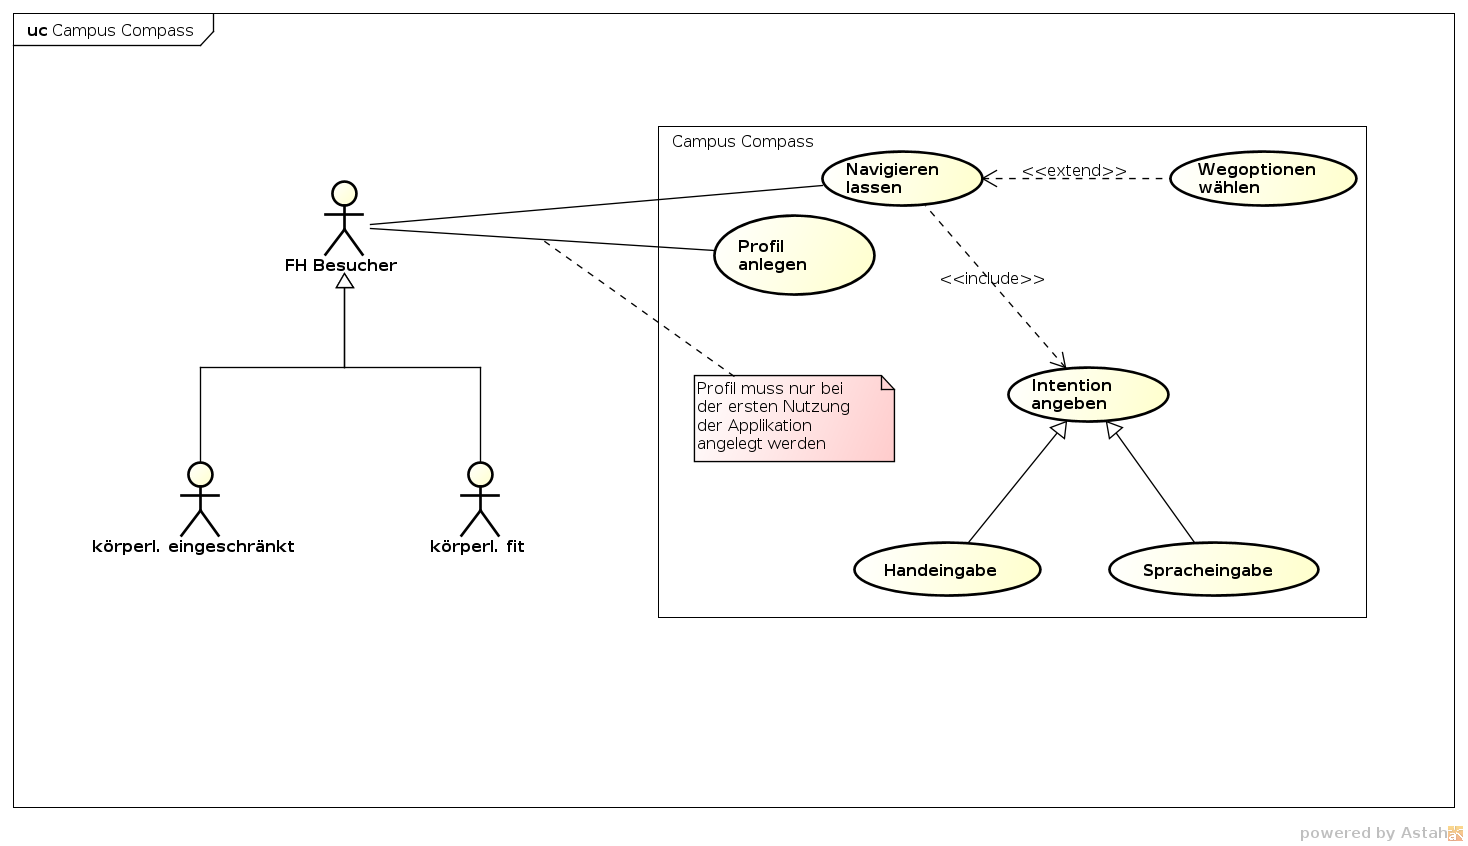
\includegraphics[width=\linewidth]{img/use-case-diagram.png}
  \label{img:use-case-diagramm}
  \caption{Use Case Diagramm}
\end{figure}

Im Use Case Diagramm ist dargestellt welche Möglichkeiten der \gls{fhbesucher} hat um mit der App (Campus Compass) zu interagieren. Es fällt auf, dass der Nutzer nur einen\footnote{Das Pflegen des Profils geschieht höchstwahrscheinlich nur bei der ersten Nutzung der Applikation} echten Use Case hat: \emph{Navigieren lassen}. Hieraus lässt sich für das Oberflächendesign ableiten, dass der Nutzer bei der Bedienung der Applikation möglichst schnell mit der \gls{navigation} beginnen möchte und eventuelle Details lieber während der \gls{navigation} einstellen wird.

\newpage

\subsubsection*{Aktivitätsdiagramme (Verhalten)}
... bieten eine standardisierte Möglichkeit, um die zuvor im Use-Case-Diagramm gezeigten Aktivitäten im Detail darzustellen. Sie zeigen die Aktionen, aus denen sich eine Aktivität zusammensetzt, sowie den Aktivitätsfluss.

\begin{figure}[hbt]
  \centering
  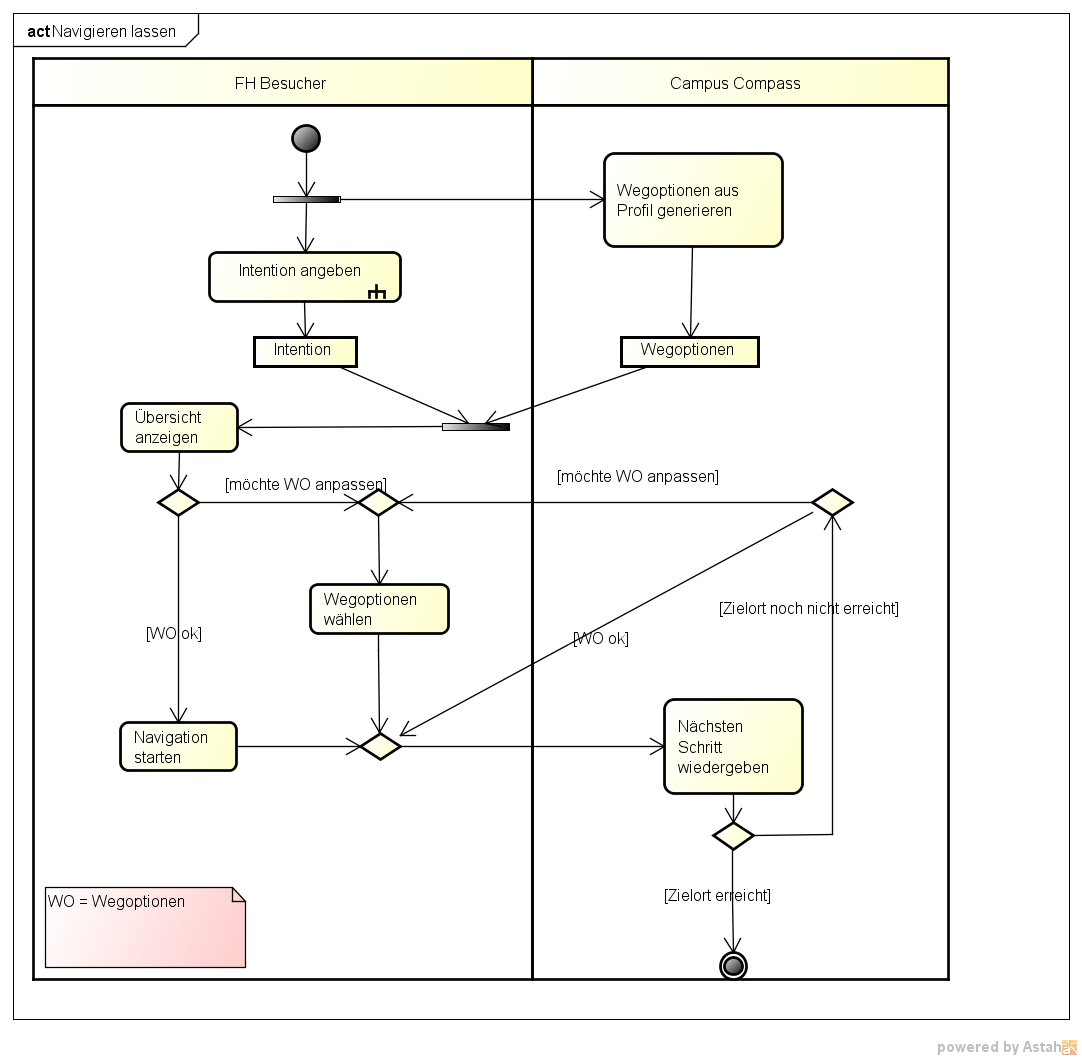
\includegraphics[width=\linewidth]{img/akt_navigieren_lassen.png}
  \label{img:akt_navigieren_lassen}
  \caption{Navigieren lassen}
\end{figure}

Das Use Case Diagramm \emph{Navigieren lassen} zeigt anschaulich den Verlauf einer \gls{weg}führung. Nach dem der \gls{fhbesucher} seine \gls{intention} der App mitgeteilt hat, bekommt er eine Übersicht seiner Auswahl angezeigt. Nun beginnt ein Kreislauf, in dem der Anwender während der gesamten \gls{weg}führung die Möglichkeit hat \gls{weg}optionen anzupassen, während die erforderlichen \gls{schritt}e um das Ziel zu erreichen nacheinander aufgeführt werden. Gibt es keinen weiteren \gls{schritt} mehr, ist der Zielort erreicht.

\begin{figure}[hbt]
  \centering
  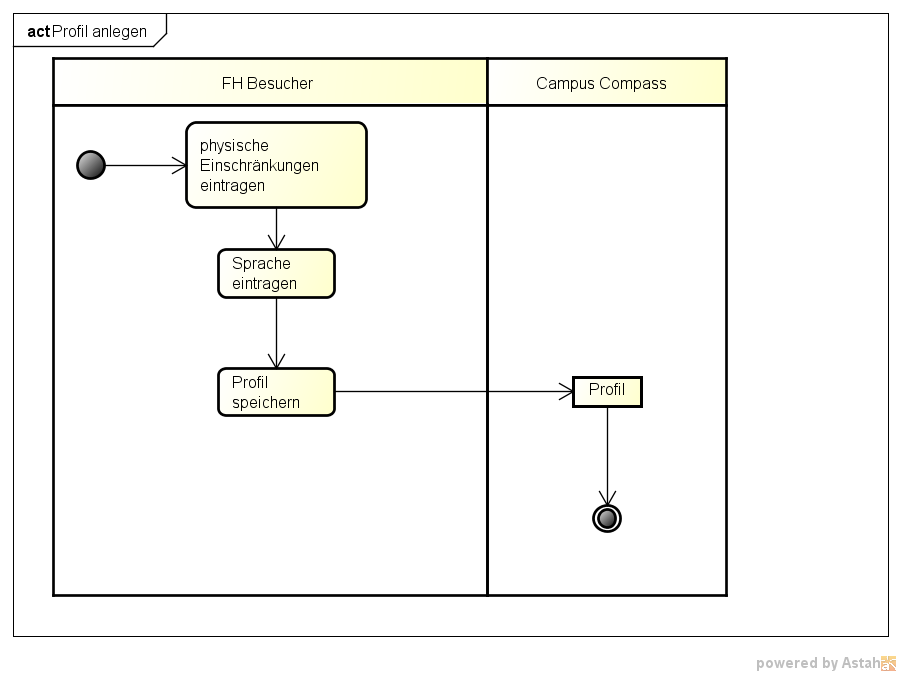
\includegraphics[width=\linewidth]{img/akt_profil_anlegen.png}
  \label{img:akt_profil_anlegen}
  \caption{Profil anlegen}
\end{figure}

\noindent Das Use Case Diagramm \emph{Profil anlegen} beschreibt den Prozess der Profil Erzeugung für den Campuss Compass durch einen \gls{fhbesucher}. Der Anwender trägt \gls{schritt} für \gls{schritt} seine physischen Einschränkungen, sowie seine bevorzugte Sprache ein, woraufhin durch das Speichern des Profils ein Profil-Objekt in der App angelegt wird.

\chapter{Interaktions-,Funktions- und Daten-Semantik}

\subsubsection*{Handlungsschema}
Dient als Brücke zwischen dem Nutzungskontext-Modell und der Interaktions-, Funktions- und Daten-Semantik.

\textbf{Attribute}
\begin{itemize}
\item Benennung der Handlung
    \begin{itemize}
    \item Navigieren lassen
    \end{itemize}
\item Kurzdefinition/Zweck
    \begin{itemize}
    \item \gls{fhbesucher} kennt den \gls{weg} zu einem \gls{ort}    nicht, an den er aufgrund eines Anliegens (einer \gls{intention}) gelangen möchte
    \end{itemize}
\item Benutzergruppen
    \begin{itemize}
    \item \gls{fhbesucher}
    \end{itemize}
\item Involvierte Dinge
    \begin{itemize}
    \item \gls{ort}
    \item \gls{weg}
    \item \gls{schritt}e
    \item \gls{tuer}en
    \item \gls{treppe}n
    \item Aufzüge
    \item Position
    \item Nutzer
    \end{itemize}
\end{itemize}

\textbf{Optionale Attribute}
\begin{itemize}
\item Auslösende Ereignis
    \begin{itemize}
    \item Der User teilt seine \gls{intention} dem System mit
    \end{itemize}
\item Vorbedingungen
    \begin{itemize}
    \item Nutzer verfügt über mobiles Endgerät
    \end{itemize}
\item Nachbedingungen bei Misserfolg
    \begin{itemize}
    \item User teilt dem System seine \gls{intention} erneut mit
    \end{itemize}
\item Invarianten
    \begin{itemize}
    \item \gls{intention} des Users ändert sich nicht (Gegensatz zum Auto Navi: Auch wenn sich die Route ändern kann ist das Ziel die Invariante. In unserem Fall kann sich auch das Ziel ändern, wenn es die \gls{intention} des Users erfüllen kann und näher liegt.)
    \end{itemize}
\item Verlaufsbedingungen
    \begin{itemize}
    \item User folgt den Anweisungen des System
    \end{itemize}
\end{itemize}

\subsubsection*{Dingschema}
\begin{center}
    \begin{tabular}{ | p{2.2cm} | c | p{2.8cm} | p{2.5cm} | c | }
    \hline
    \textbf{Benennung des Ding} & \textbf{Kurzdefinition} & \textbf{Merkmale} & \textbf{Beziehungen zu anderen Dingen} & \textbf{Zustandsraum} \\ \hline
    \gls{ort} & (siehe Glossar) & Position, Bedeutung, Bezeichnung & & geöffnet/nicht geöffnet \\ \hline
    \gls{weg} & (siehe Glossar) & Startort, Zielort, \gls{schritt}e & Verbindet zwei \gls{ort}e & gesperrt/nicht gesperrt\\ \hline 
    \gls{schritt} & (siehe Glossar) & Startposition, Endposition, Länge, Begehbarkeit & Ein \gls{schritt} ist Teil eines \gls{weg}es &\\ \hline 
    \gls{tuer}en & (siehe Glossar) & Begehbarkeit & Teil eines \gls{schritt}s & verschlossen/geöffnet\\ \hline 
    \gls{treppe}n, Aufzüge & (siehe Glossar) & Etagen, Begehbarkeit, Länge & Besondere \gls{schritt}e eines \gls{weg}es & In/Außer Betrieb\\ \hline 
    Position & (siehe Glossar) & Koordinaten (X,Y,Z) & \gls{ort}, \gls{weg}, \gls{schritt} &\\ \hline 
    \gls{fhbesucher} & (siehe Glossar) & Alter, Fitness, Sprache & Position, \gls{ort} & still, in Bewegung\\ \hline 
    \end{tabular}
\end{center}
\chapter{Conceptual Design}
Ein erstes Design für die Benutzeroberfläche wurde mit dem Mockup Tool \textit{Balsamiq} entwickelt. Hierbei ging es primär darum Unstimmigkeiten und grobe Fehleinschätzungen auszumerzen, um anschließend einen funktionalen Prototypen entwickeln zu können. Mehr oder weniger parallel wurden auch schon Mock-Ups mit Hilfe von HTML erzeugt, welche den Vorteil hatten, später weiter genutzt werden zu können, da für die Umsetzung der App hauptsächlich HTML5 und JavaScript zum Einsatz kam.

Auf den folgenden Bildern sind die \textit{Balsamiq} Mock-Ups und die ggf. verschiedenen Versionen der App Umsetzung bzw. der HTML Mock-Ups zu sehen:

\subsubsection*{Mockups}
\begin{figure}[ht]
\centering
\begin{minipage}[b]{.5\textwidth}
  \centering
  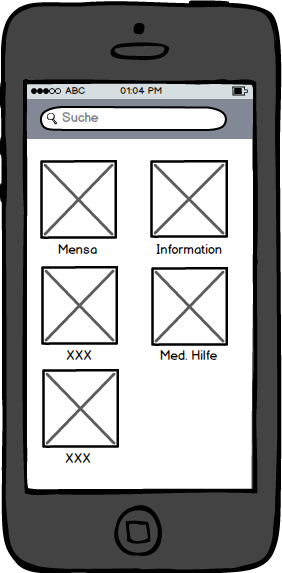
\includegraphics[width=.8\linewidth]{img/menu-mockup.png}
  \label{img:menu-mockup}
  \captionof{figure}{Menü Mockup}
\end{minipage}%
\begin{minipage}[b]{.5\textwidth}
  \centering
  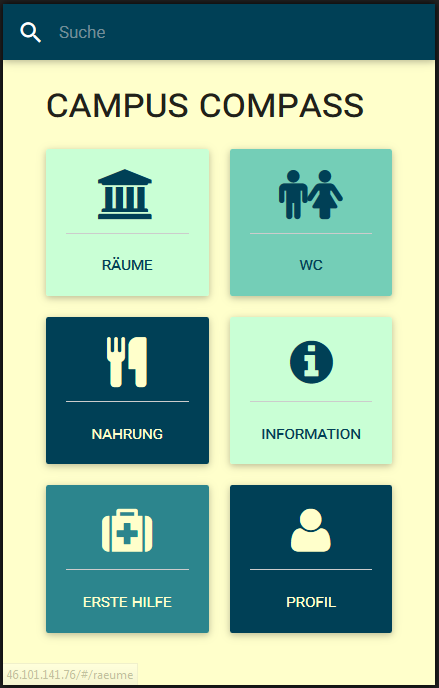
\includegraphics[width=.8\linewidth]{img/menu.png}
  \label{img:menu-first-draft}
  \captionof{figure}{Erster Entwurf Menü}
\end{minipage}
\end{figure}

\begin{figure}[ht]
\centering
\begin{minipage}[b]{.5\textwidth}
  \centering
  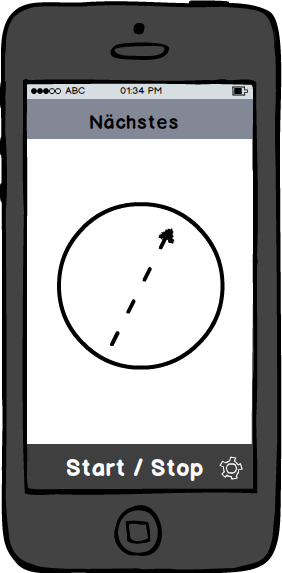
\includegraphics[width=.8\linewidth]{img/navigation-mockup.png}
  \label{img:navigation-mockup}
  \captionof{figure}{Navigation Mockup}
\end{minipage}%
\begin{minipage}[b]{.5\textwidth}
  \centering
  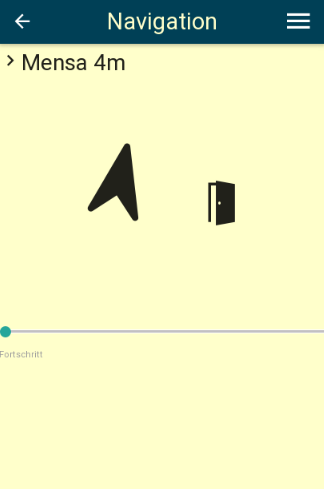
\includegraphics[width=.8\linewidth]{img/navigation.png}
  \label{img:navigation-first-draft}
  \captionof{figure}{Erster Entwurf Navigation}
\end{minipage}
\begin{minipage}[b]{.5\textwidth}
  \centering
  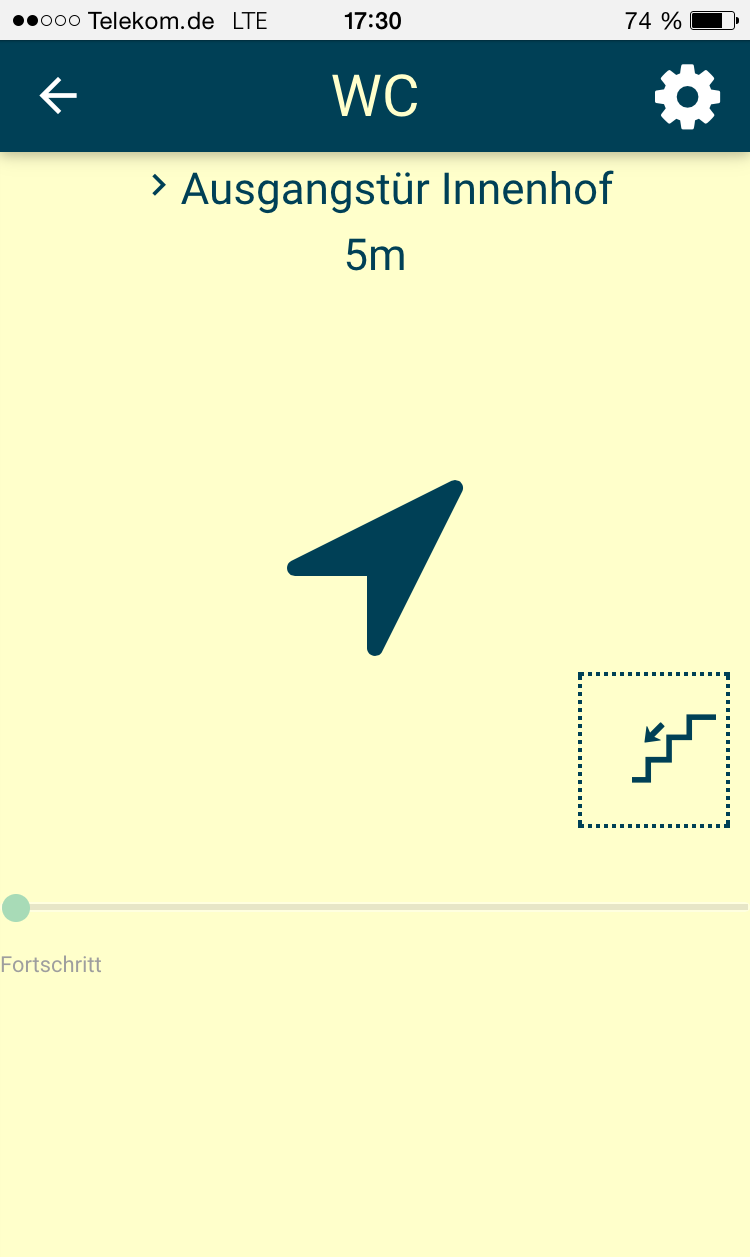
\includegraphics[width=.8\linewidth]{img/navigation2.png}
  \label{img:navigation-second-draft}
  \captionof{figure}{Aktuelle Ansicht Navigation}
\end{minipage}
\end{figure}

\begin{figure}[ht]
\centering
\begin{minipage}[b]{.5\textwidth}
  \centering
  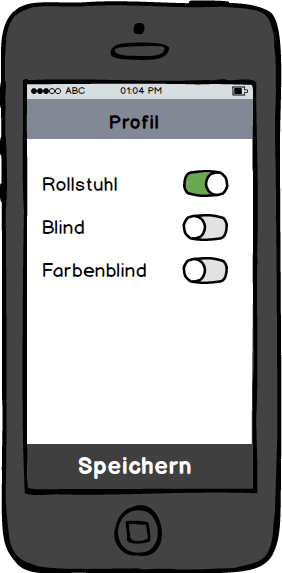
\includegraphics[width=.8\linewidth]{img/profil-mockup.png}
  \label{img:profil-mockup}
  \captionof{figure}{Profil Mockup}
\end{minipage}%
\begin{minipage}[b]{.5\textwidth}
  \centering
  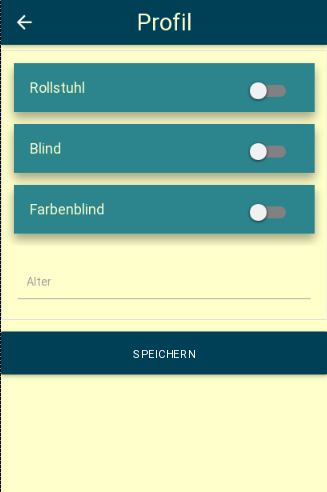
\includegraphics[width=.8\linewidth]{img/profil.png}
  \label{img:profil-first-draft}
  \captionof{figure}{Erster Entwurf Profil}
\end{minipage}
\end{figure}

\begin{figure}[ht]
\centering
\begin{minipage}[b]{.5\textwidth}
  \centering
  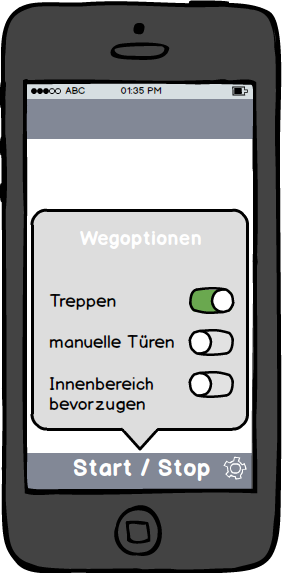
\includegraphics[width=.8\linewidth]{img/wegoptionen-mockup.png}
  \label{img:wegoptionen-mockup}
  \captionof{figure}{Wegoptionen Mockup}
\end{minipage}%
\begin{minipage}[b]{.5\textwidth}
  \centering
  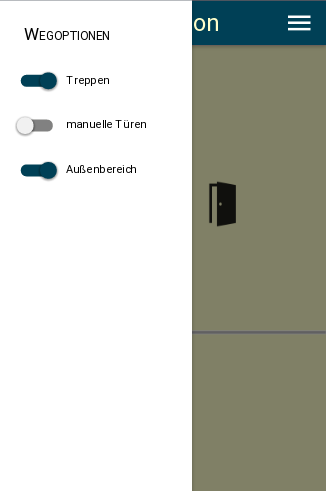
\includegraphics[width=.8\linewidth]{img/wegoptionen.png}
  \label{img:wegoptionen-first-draft}
  \captionof{figure}{Erster Entwurf Wegoptionen}
\end{minipage}
\end{figure}
\chapter{Objekt-Semantik}

\subsubsection*{Klassendiagramm (Struktur)}
... bieten eine standardisierte Möglichkeit um die zuvor genannten Nutzer und ihre Use Cases sowie die Beziehungen zwischen Use Cases untereinander darzustellen.

\begin{figure}[hbt]
  \centering
  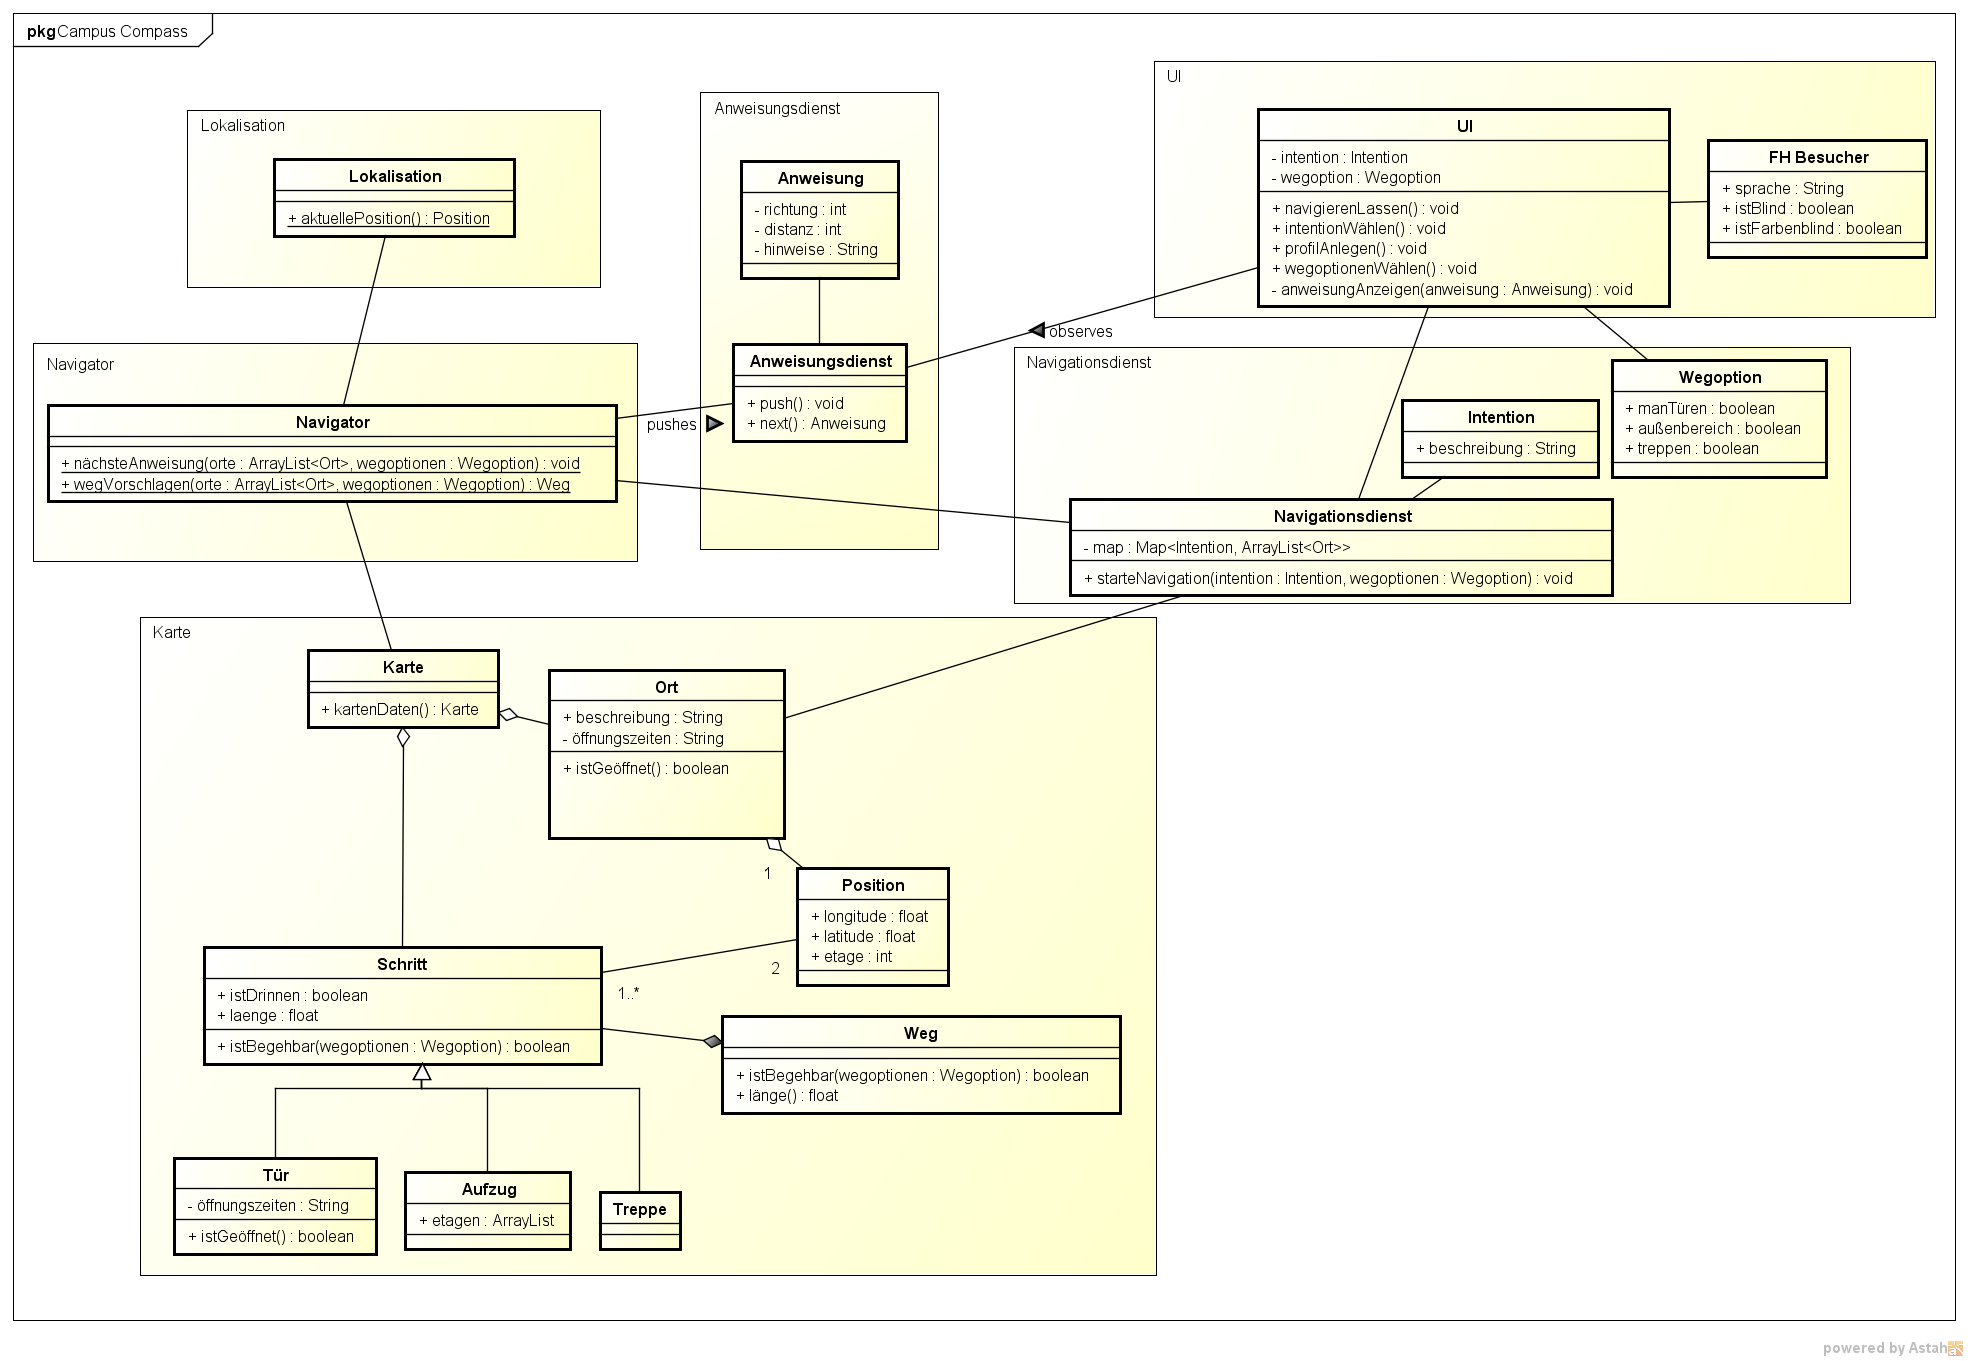
\includegraphics[width=\linewidth]{img/klassendiagramm.png}
  \label{img:klassendiagramm}
  \caption{Klassendiagramm}
\end{figure}

\subsubsection*{Zustandsdiagramm (Verhalten)}
... bieten eine standardisierte Möglichkeit um die zuvor genannten Nutzer und ihre Use Cases sowie die Beziehungen zwischen Use Cases untereinander darzustellen.

\begin{figure}[hbt]
  \centering
  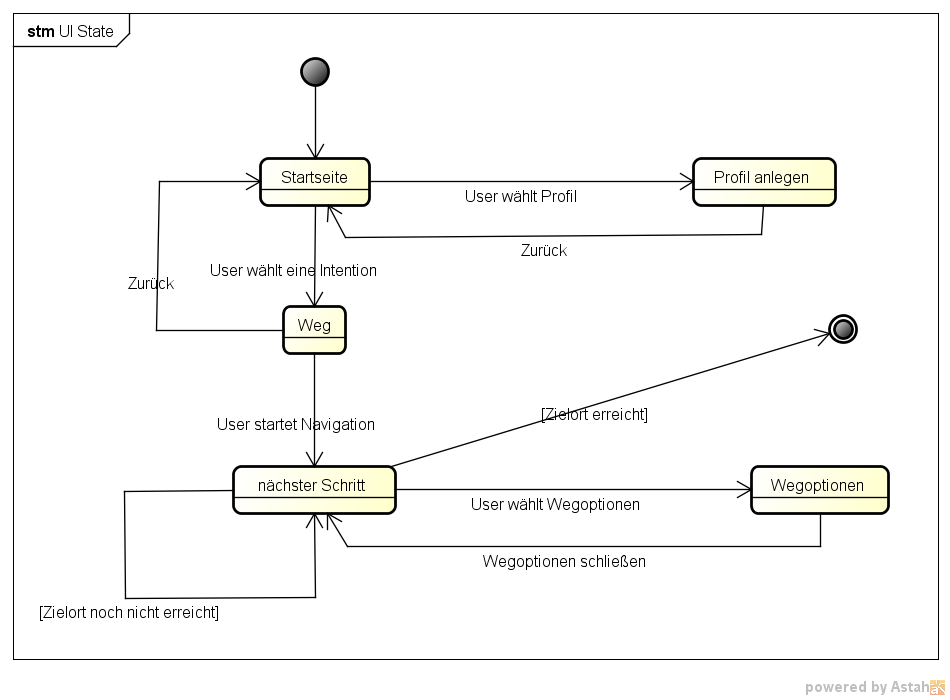
\includegraphics[width=\linewidth]{img/zustandsdiagramm.png}
  \label{img:zustandsdiagramm}
  \caption{Zustandsdiagramm}
\end{figure}

\subsubsection*{Sequenzdiagramm (Verhalten)}
... bieten eine standardisierte Möglichkeit um die zuvor genannten Nutzer und ihre Use Cases sowie die Beziehungen zwischen Use Cases untereinander darzustellen.

\begin{figure}[hbt]
  \centering
  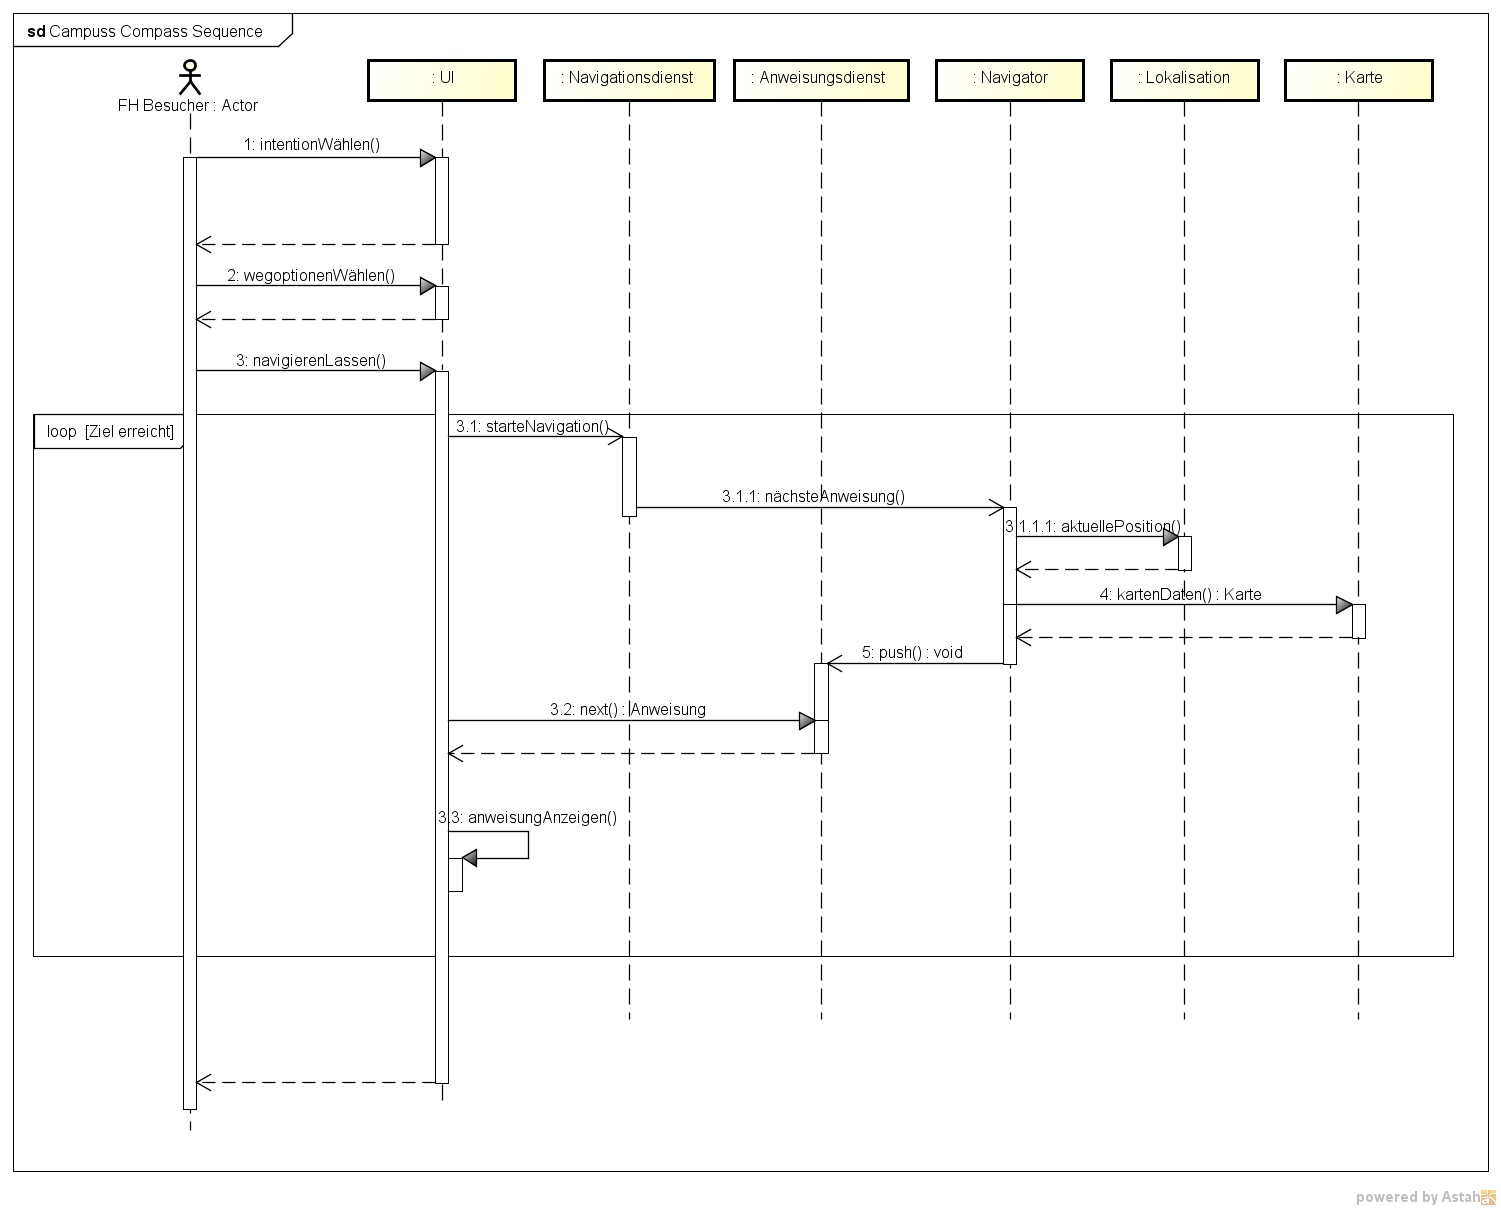
\includegraphics[width=\linewidth]{img/sequenzdiagramm.png}
  \label{img:sequenzdiagramm}
  \caption{Sequenzdiagramm}
\end{figure}
\chapter{Komponentensemantik}
ST: Komponenten-Realisierungssemantik: Komponenten-Diagramm mit
interner Klassenstruktur;
Komponenten-Benutztsemantik: Komponenten-Diagramm mit expliziten
Schnittstellen ohne interne Klassenstruktur;

\subsubsection*{Komponentendiagramm}
... zeigt die austauschbaren Komponenten inkl. ihrer Schnittstellen im System. Es wird zwischen angebotenen und genutzten Schnittstellen unterschieden. Eine Komponente kann dabei aus mehreren Klassen des Klassendiagramms bestehen.

\textbf{externe Sicht}
(Der interne Inhalt der Komponente wird bleibt in dieser Darstellung verborgen.)
\begin{figure}[hbt]
  \centering
  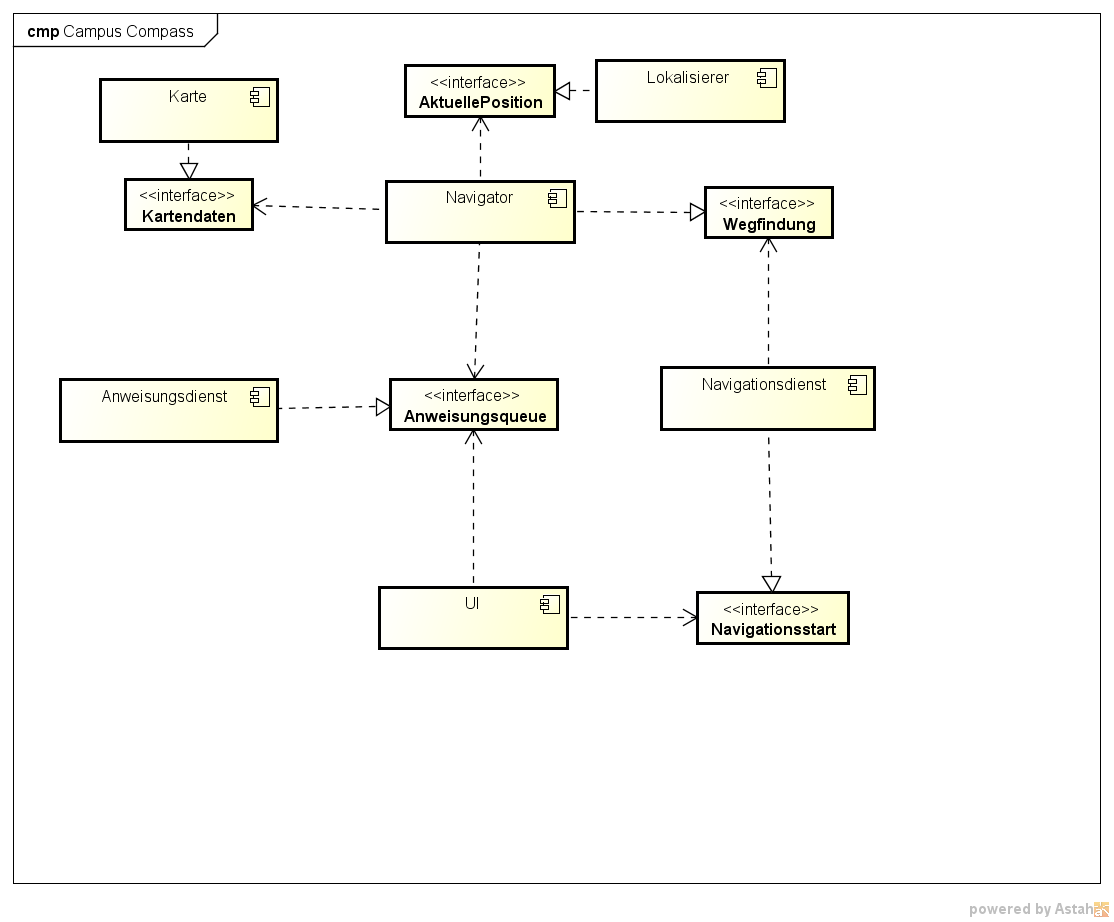
\includegraphics[width=\linewidth]{img/komponentendiagramm.png}
  \label{img:komponentendiagramm}
  \caption{Komponentendiagramm}
\end{figure}

\textbf{interne Sicht}
siehe Klassendiagramm...
\chapter{Usability Test}

\section{Vorbereitung}

\subsubsection*{Was ist das Ziel?}
Unser Ziel ist es, den Nutzer zu seinem Ziel zu führen, das er entweder über die direkte Eingabe der Raumnummer oder über eine Eingabe der \gls{intention} wählt.
Dabei achten wir vor allem darauf, dass die Bedienung effektiv, effizient und zufriedenstellend abläuft.
\subsubsection*{Testplan}
\begin{itemize}
\item \textbf{Teilnehmer:} Mara Braun, Fabian Hardt, Thomas Kopp
\item \textbf{Methoden:} Video, Log-Files, Lautes Denken, Eye-Tracking, Fragebogen
\item \textbf{Aufgaben:} Siehe unten
\item \textbf{Testumgebung:} Mobiles Endgerät des Nutzers (Smartphone oder Tablet), Anwendung wird auf Server deployt
\item \textbf{Rolle und Aufgaben des Test-Moderators:} Der Moderator weist die Testperson in die Aufgabe ein und steht bei Fragen zur Verfügung. Vor Beginn des Tests sollten die Kameras eingestellt und dem Tester das Eye-Tracking sowie das Vorgehen des Tests erläutert werden.
\item \textbf{Testdaten und Bewertungsmaße:} Schwerwiegende Probleme, die die Benutzung verhindern. Mittelschwere Probleme, die die Benutzung erschweren. Leichtwiegende Probleme, die das Design und persönliche Präferenzen betreffen.
\item \textbf{Bericht, Präsentation:} Bericht wird aus Fragebogen generiert.
\end{itemize}

\newpage

\subsubsection*{Testaufgabe}
\begin{itemize}
\item \textbf{Einleitung:} Wir zeigen der Testperson erst die Startseite und fragen sie nach ihren Erwartungen und Eindrücken.
\begin{enumerate}
\item Du verlässt die Vorlesung und musst dringend auf Toilette. Wie würdest du navigieren?
\item Du hast in 5 Minuten Vorlesung, aber vergessen wo \gls{raum} 2230 ist. Wie würdest du vorgehen, um den \gls{raum} zu finden?
\item Du hast dir letzte Woche ein Bein gebrochen und bist nun auf Krücken unterwegs. Du möchtest von den Tischtennisplatten herüber zur \gls{mensa}, um Mittag zu essen. Da es aber draußen Hunde und Katzen regnet, möchtest du den Außenbereich so lange wie möglich meiden. Wie wirst du die App benutzen?
\item Du möchtest in die Sprechstunde von Prof. Klocke, kennst seine Büroraumnummer aber nicht, wie kannst du dich zu seinem Büro navigieren lassen?
\item Kienbaum veranstaltet seine Preisverleihung im gesponsorten Vorlesungssaal, du möchtest an dir die Preisverleihung ansehen, wie findest du heraus wo der Kienbaum Saal ist?
\end{enumerate}
\newpage
\item \textbf{Material und Systemzustand}
\begin{itemize}
\item Smartphone oder PC
\item ggf. Eingabegeräte (falls PC)
\item Eye-Tracking-Kamera
\item Videokamera
\item Fragebogen
\item App zeigt Startseite
\end{itemize}
\item \textbf{Beschreibung der erfolgreichen Lösung}
\begin{enumerate}
\item Der Nutzer klickt auf der Startseite des Campus Compass sofort auf die Karte "`WC"'' und lässt sich navigieren.
\item Die Testperson befindet sich auf der Startseite der \gls{navigation} und klickt auf "`\gls{information}"', um sich navigieren zu lassen.
Alternativ: Der Nutzer benutzt den Header, um den \gls{raum} einzugeben und lässt sich von da an navigieren.
\item Der Tester beginnt indem auf die Karte "`Nahrung"'' klickt, um sich zur \gls{mensa} navigieren zu lassen. Auf der nächsten Ansicht wählt er in der rechten oberen Ecke die Optionen und stellt "`Lift bevorzugen"', "`man. \gls{tuer}en"'' und "`Innenbereich"'' an. Nun kann die \gls{navigation} beginnen.
Alternativ: Der Nutzer beginnt, indem er versucht sich ein Profil einzurichten, um seine Bedürfnisse anzupassen.
\end{enumerate}
\end{itemize}
\newpage
\subsubsection*{Fragebogen zur Usability}
Im folgenden zu sehen ist der Fragebogen, welcher den Probanden jeweils nach Abschluss des Tests zum ausfüllen vorgelegt wurde. Die Ergebnisse des Test werden im Anschluss zusammengefasst.

\begin{center}
    \begin{tabular}{ | c | c | c | }
    \hline
    \textbf{Bedienung} & \textbf{Bewertung} &  \\ \hline
    einfach & \degree \degree \degree \degree \degree & kompliziert \\ \hline
    angenehm & \degree \degree \degree \degree \degree & unangenehm \\  \hline
    originell & \degree \degree \degree \degree \degree & konventionell \\ \hline
    praktisch & \degree \degree \degree \degree \degree & unpraktisch \\ \hline
    voraussagbar & \degree \degree \degree \degree \degree & unberechenbar \\ \hline
    intuitiv & \degree \degree \degree \degree \degree & unintuitiv \\ \hline
    \end{tabular}
\end{center}

\begin{center}
    \begin{tabular}{ | c | c | c | }
    \hline
    \textbf{Design} & \textbf{Bewertung} &  \\ \hline
    angenehm & \degree \degree \degree \degree \degree & unangenehm \\ \hline
    originell & \degree \degree \degree \degree \degree & konventionell \\  \hline
    schön & \degree \degree \degree \degree \degree & hässlich \\ \hline
    sympathisch & \degree \degree \degree \degree \degree & unsympathisch \\ \hline
    einladend & \degree \degree \degree \degree \degree & zurückweisend \\ \hline
    modern & \degree \degree \degree \degree \degree & obsolet \\ \hline
    \end{tabular}
\end{center}
\vspace{1cm}
\noindent{
\vspace{2cm}
Aus welchen Gründen würdest du die App auch im Alltag nutzen oder nicht nutzen? \\
\vspace{2cm}
Würdest du die App Erstsemestern weiterempfehlen? \\
\vspace{2cm}
Was hat dir gut gefallen? \\
\vspace{2cm}
Was könnten wir verbessern? \\
}

\section{Evaluationsergebnisse}

\subsubsection*{Rahmenbedingungen}
\textbf{Probanden:} Thomas Kopp (iOS-User), Mara Braun (Android-User), Fabian Hardt (iOS-User)

\textbf{Testgerät:} Samsung Galaxy Note (Android)

\textbf{Methoden:} Eye-Tracking, Lautes Denken, Evaluationsbogen, Befragung

\textbf{Aufgaben:} siehe Usability Testplan

\subsubsection*{Vorgehensweise}

Nach einer kurzen Einführung und Aufklärung des Test durch den Moderator, wurde dem jeweiligen Probanden eine Aufgabe (entnommen aus dem Testplan) laut vorgelesen. Der Proband wurde gebeten, bei all seinen Handlungen laut zu denken, wodurch im Falle einer Verwirrung oder Unklarheit im Bezug auf die Aufgabe mit der App die Beobachter diese unmittelbar erfassen konnten. Um eine realitätsnahe Situation herzustellen, wurde wenn nicht zwingend nötig, auf Hilfe durch den Moderator verzichtet. In der Ausgangssituation zeigt die App immer die Startseite.

Im Anschluss des Tests wurde jeder Proband gebeten einen Evaluationsbogen auszufüllen. Darauf folgend, haben wir noch die Möglichkeit wahrgenommen, dem Testanwender direkt zur Anwendung, seinen Erfahrungen, seinen Problemen und Anregungen zu befragen.
\newpage
\subsubsection*{Ergebnisse}

Es ist jeden Testanwender gelungen, die ihm aufgetragenen Aufgaben in angemessener Zeit ohne größere Hilfestellungen zu lösen.

Sowohl bei der Beobachtung, sowie als auch bei der anschließenden Befragung, kristallisierten sich folgende Dinge heraus:
\begin{itemize}
    \item Die Kachel “\gls{information}” lässt einen zu großen Interpretationsspielraum offen, die User unterschieden zwischen \gls{information}en über die App als solche, \gls{information}en über den Campus und \gls{information} in Form eines \gls{ort}en (z.B. Rezeption)
    \begin{itemize}
        \item Lösungsvorschlag: Umbenennung oder Entfernung der Kachel, sowie ggf. des Kachel-Symbols
        \item Gewichtung: Problem Mittelschwer, da Usability und Verständnis beeinflusst. Lösung einfach
    \end{itemize}
    \item Die Kachel “Profil” suggerierte den Probanden die Einstellungen von Wegoptionen. Wurde dem Anwender aufgetragen, Wegoptionen anzupassen, versuchte er stets diese im “Profil” anzupassen, statt die in der gestarteten \gls{navigation} gebotene Funktion zu nutzen
    \begin{itemize}
        \item Lösungsvorschlag: Profil entfernen oder Wegoptionen basierend auf dem Profil automatisch einstellen und dem User diese Funktion als Hinweis im “Profil” anzeigen
        \item Gewichtung: Problem Mittelschwer, da Usability und Verständnis beeinflusst. Lösung einfach
    \end{itemize}
    \item Die in der App verfügbare Multisuchfunktion und der Raumfilter wurden jeweils nur rar genutzt, dies stellt jedoch kein kritisches Usability Problem dar, wird durch das Fehlen von Testdaten provoziert und bieten dem User verschiedene Möglichkeiten die App zu bedienen
    \begin{itemize}
        \item Lösungsvorschlag: Weitere (Test)-Daten hinzufügen
        \item Gewichtung: Problem Leichtwiegend, da die Nutzung nicht direkt behindert wird
    \end{itemize}
\end{itemize}
\newpage
\subsubsection*{Auswertung der Evaluationsbögen}

Die Auswertung der Evaluationsbögen ergab folgendes:

Insgesamt wurden zwei Probanden zur Bedienung und dem Design befragt.
Bei der Bedienung überzeugt unsere Applikation vor allem durch eine einfache, angenehme und praktische Weise. Durch das modulare System, dass keine tiefen Schachtelungen enthält, findet man durch wenige Eingaben zu seinem Ziel.
Des weiteren sind die Funktionen voraussagbar und intuitiv -mit Ausnahme des Profils und der \gls{information}. Dadurch gab es leichte Abstriche.

Das Design war für beide Nutzer ansprechend gestaltet und konnte mit einer modernen Oberfläche angenehm und einladend wirken.

Dass die App auch klar im Alltag genutzt werden würde, zeigte sich durch die offenen Fragen am Ende. Vor allem in "`großen Gebäuden, in denen man sich nicht auskennt"' und für "`Räume und Toiletten"' ist diese App praktisch.
Beide Probanden würden die App uneingeschränkt weiterempfehlen.

Verbesserungsbedarf besteht bei der Aussagekraft der Menüpunkte \gls{information} und des Profils, das Voreinstellungen für die Wegoptionen bieten sollte.

Insgesamt überzeugte unser Campus Compass mit einem schönen, intuitiven Design und der einfachen und unkomplizierten Bedienung.
\chapter{Komponentenübergreifendes Systemverhalten im Nutzungskontext}
ST: Sequenzdiagramm mit den Komponenteninteraktionen für jeden Use
Case
MCI: Evaluierungsergebnisse
\chapter{Resümee}
Projektfazit, Schwerpunkte in MCI/ST2, Methodeneinschätzung, -
abgrenzung

\textbf{Portfolio, was muss rein?}
  Idee/Vorgehensweise(was? warum?)/Methodik
  Problem-und Kontextanalyse
  Benutzermodellierung
  Aufgabenmodellierung
  User Needs
  Usability Testplan
  Bericht der Evaluation/Tests
  Verbesserungsvorschläge
  Paper Prototype
  Aktivitätsszenario
  Wireframes/Computer based Prototypes
  Fazit

  Quelle: MCI 5 Usability Evaluation (Seite 37)
\end{document}
